\documentclass{ximera}

%\usepackage{todonotes}
%\usepackage{mathtools} %% Required for wide table Curl and Greens
%\usepackage{cuted} %% Required for wide table Curl and Greens
\newcommand{\todo}{}

\usepackage{esint} % for \oiint
\ifxake%%https://math.meta.stackexchange.com/questions/9973/how-do-you-render-a-closed-surface-double-integral
\renewcommand{\oiint}{{\large\bigcirc}\kern-1.56em\iint}
\fi


\graphicspath{
  {./}
  {ximeraTutorial/}
  {basicPhilosophy/}
  {functionsOfSeveralVariables/}
  {normalVectors/}
  {lagrangeMultipliers/}
  {vectorFields/}
  {greensTheorem/}
  {shapeOfThingsToCome/}
  {dotProducts/}
  {partialDerivativesAndTheGradientVector/}
  {../productAndQuotientRules/exercises/}
  {../normalVectors/exercisesParametricPlots/}
  {../continuityOfFunctionsOfSeveralVariables/exercises/}
  {../partialDerivativesAndTheGradientVector/exercises/}
  {../directionalDerivativeAndChainRule/exercises/}
  {../commonCoordinates/exercisesCylindricalCoordinates/}
  {../commonCoordinates/exercisesSphericalCoordinates/}
  {../greensTheorem/exercisesCurlAndLineIntegrals/}
  {../greensTheorem/exercisesDivergenceAndLineIntegrals/}
  {../shapeOfThingsToCome/exercisesDivergenceTheorem/}
  {../greensTheorem/}
  {../shapeOfThingsToCome/}
  {../separableDifferentialEquations/exercises/}
  {vectorFields/}
}

\newcommand{\mooculus}{\textsf{\textbf{MOOC}\textnormal{\textsf{ULUS}}}}

\usepackage{tkz-euclide}\usepackage{tikz}
\usepackage{tikz-cd}
\usetikzlibrary{arrows}
\tikzset{>=stealth,commutative diagrams/.cd,
  arrow style=tikz,diagrams={>=stealth}} %% cool arrow head
\tikzset{shorten <>/.style={ shorten >=#1, shorten <=#1 } } %% allows shorter vectors

\usetikzlibrary{backgrounds} %% for boxes around graphs
\usetikzlibrary{shapes,positioning}  %% Clouds and stars
\usetikzlibrary{matrix} %% for matrix
\usepgfplotslibrary{polar} %% for polar plots
\usepgfplotslibrary{fillbetween} %% to shade area between curves in TikZ
\usetkzobj{all}
\usepackage[makeroom]{cancel} %% for strike outs
%\usepackage{mathtools} %% for pretty underbrace % Breaks Ximera
%\usepackage{multicol}
\usepackage{pgffor} %% required for integral for loops



%% http://tex.stackexchange.com/questions/66490/drawing-a-tikz-arc-specifying-the-center
%% Draws beach ball
\tikzset{pics/carc/.style args={#1:#2:#3}{code={\draw[pic actions] (#1:#3) arc(#1:#2:#3);}}}



\usepackage{array}
\setlength{\extrarowheight}{+.1cm}
\newdimen\digitwidth
\settowidth\digitwidth{9}
\def\divrule#1#2{
\noalign{\moveright#1\digitwidth
\vbox{\hrule width#2\digitwidth}}}





\newcommand{\RR}{\mathbb R}
\newcommand{\R}{\mathbb R}
\newcommand{\N}{\mathbb N}
\newcommand{\Z}{\mathbb Z}

\newcommand{\sagemath}{\textsf{SageMath}}


%\renewcommand{\d}{\,d\!}
\renewcommand{\d}{\mathop{}\!d}
\newcommand{\dd}[2][]{\frac{\d #1}{\d #2}}
\newcommand{\pp}[2][]{\frac{\partial #1}{\partial #2}}
\renewcommand{\l}{\ell}
\newcommand{\ddx}{\frac{d}{\d x}}

\newcommand{\zeroOverZero}{\ensuremath{\boldsymbol{\tfrac{0}{0}}}}
\newcommand{\inftyOverInfty}{\ensuremath{\boldsymbol{\tfrac{\infty}{\infty}}}}
\newcommand{\zeroOverInfty}{\ensuremath{\boldsymbol{\tfrac{0}{\infty}}}}
\newcommand{\zeroTimesInfty}{\ensuremath{\small\boldsymbol{0\cdot \infty}}}
\newcommand{\inftyMinusInfty}{\ensuremath{\small\boldsymbol{\infty - \infty}}}
\newcommand{\oneToInfty}{\ensuremath{\boldsymbol{1^\infty}}}
\newcommand{\zeroToZero}{\ensuremath{\boldsymbol{0^0}}}
\newcommand{\inftyToZero}{\ensuremath{\boldsymbol{\infty^0}}}



\newcommand{\numOverZero}{\ensuremath{\boldsymbol{\tfrac{\#}{0}}}}
\newcommand{\dfn}{\textbf}
%\newcommand{\unit}{\,\mathrm}
\newcommand{\unit}{\mathop{}\!\mathrm}
\newcommand{\eval}[1]{\bigg[ #1 \bigg]}
\newcommand{\seq}[1]{\left( #1 \right)}
\renewcommand{\epsilon}{\varepsilon}
\renewcommand{\phi}{\varphi}


\renewcommand{\iff}{\Leftrightarrow}

\DeclareMathOperator{\arccot}{arccot}
\DeclareMathOperator{\arcsec}{arcsec}
\DeclareMathOperator{\arccsc}{arccsc}
\DeclareMathOperator{\si}{Si}
\DeclareMathOperator{\scal}{scal}
\DeclareMathOperator{\sign}{sign}


%% \newcommand{\tightoverset}[2]{% for arrow vec
%%   \mathop{#2}\limits^{\vbox to -.5ex{\kern-0.75ex\hbox{$#1$}\vss}}}
\newcommand{\arrowvec}[1]{{\overset{\rightharpoonup}{#1}}}
%\renewcommand{\vec}[1]{\arrowvec{\mathbf{#1}}}
\renewcommand{\vec}[1]{{\overset{\boldsymbol{\rightharpoonup}}{\mathbf{#1}}}\hspace{0in}}

\newcommand{\point}[1]{\left(#1\right)} %this allows \vector{ to be changed to \vector{ with a quick find and replace
\newcommand{\pt}[1]{\mathbf{#1}} %this allows \vec{ to be changed to \vec{ with a quick find and replace
\newcommand{\Lim}[2]{\lim_{\point{#1} \to \point{#2}}} %Bart, I changed this to point since I want to use it.  It runs through both of the exercise and exerciseE files in limits section, which is why it was in each document to start with.

\DeclareMathOperator{\proj}{\mathbf{proj}}
\newcommand{\veci}{{\boldsymbol{\hat{\imath}}}}
\newcommand{\vecj}{{\boldsymbol{\hat{\jmath}}}}
\newcommand{\veck}{{\boldsymbol{\hat{k}}}}
\newcommand{\vecl}{\vec{\boldsymbol{\l}}}
\newcommand{\uvec}[1]{\mathbf{\hat{#1}}}
\newcommand{\utan}{\mathbf{\hat{t}}}
\newcommand{\unormal}{\mathbf{\hat{n}}}
\newcommand{\ubinormal}{\mathbf{\hat{b}}}

\newcommand{\dotp}{\bullet}
\newcommand{\cross}{\boldsymbol\times}
\newcommand{\grad}{\boldsymbol\nabla}
\newcommand{\divergence}{\grad\dotp}
\newcommand{\curl}{\grad\cross}
%\DeclareMathOperator{\divergence}{divergence}
%\DeclareMathOperator{\curl}[1]{\grad\cross #1}
\newcommand{\lto}{\mathop{\longrightarrow\,}\limits}

\renewcommand{\bar}{\overline}

\colorlet{textColor}{black}
\colorlet{background}{white}
\colorlet{penColor}{blue!50!black} % Color of a curve in a plot
\colorlet{penColor2}{red!50!black}% Color of a curve in a plot
\colorlet{penColor3}{red!50!blue} % Color of a curve in a plot
\colorlet{penColor4}{green!50!black} % Color of a curve in a plot
\colorlet{penColor5}{orange!80!black} % Color of a curve in a plot
\colorlet{penColor6}{yellow!70!black} % Color of a curve in a plot
\colorlet{fill1}{penColor!20} % Color of fill in a plot
\colorlet{fill2}{penColor2!20} % Color of fill in a plot
\colorlet{fillp}{fill1} % Color of positive area
\colorlet{filln}{penColor2!20} % Color of negative area
\colorlet{fill3}{penColor3!20} % Fill
\colorlet{fill4}{penColor4!20} % Fill
\colorlet{fill5}{penColor5!20} % Fill
\colorlet{gridColor}{gray!50} % Color of grid in a plot

\newcommand{\surfaceColor}{violet}
\newcommand{\surfaceColorTwo}{redyellow}
\newcommand{\sliceColor}{greenyellow}




\pgfmathdeclarefunction{gauss}{2}{% gives gaussian
  \pgfmathparse{1/(#2*sqrt(2*pi))*exp(-((x-#1)^2)/(2*#2^2))}%
}


%%%%%%%%%%%%%
%% Vectors
%%%%%%%%%%%%%

%% Simple horiz vectors
\renewcommand{\vector}[1]{\left\langle #1\right\rangle}


%% %% Complex Horiz Vectors with angle brackets
%% \makeatletter
%% \renewcommand{\vector}[2][ , ]{\left\langle%
%%   \def\nextitem{\def\nextitem{#1}}%
%%   \@for \el:=#2\do{\nextitem\el}\right\rangle%
%% }
%% \makeatother

%% %% Vertical Vectors
%% \def\vector#1{\begin{bmatrix}\vecListA#1,,\end{bmatrix}}
%% \def\vecListA#1,{\if,#1,\else #1\cr \expandafter \vecListA \fi}

%%%%%%%%%%%%%
%% End of vectors
%%%%%%%%%%%%%

%\newcommand{\fullwidth}{}
%\newcommand{\normalwidth}{}



%% makes a snazzy t-chart for evaluating functions
%\newenvironment{tchart}{\rowcolors{2}{}{background!90!textColor}\array}{\endarray}

%%This is to help with formatting on future title pages.
\newenvironment{sectionOutcomes}{}{}



%% Flowchart stuff
%\tikzstyle{startstop} = [rectangle, rounded corners, minimum width=3cm, minimum height=1cm,text centered, draw=black]
%\tikzstyle{question} = [rectangle, minimum width=3cm, minimum height=1cm, text centered, draw=black]
%\tikzstyle{decision} = [trapezium, trapezium left angle=70, trapezium right angle=110, minimum width=3cm, minimum height=1cm, text centered, draw=black]
%\tikzstyle{question} = [rectangle, rounded corners, minimum width=3cm, minimum height=1cm,text centered, draw=black]
%\tikzstyle{process} = [rectangle, minimum width=3cm, minimum height=1cm, text centered, draw=black]
%\tikzstyle{decision} = [trapezium, trapezium left angle=70, trapezium right angle=110, minimum width=3cm, minimum height=1cm, text centered, draw=black]


\outcome{Use limits to find the slope of the tangent line at a point.}
\outcome{Understand the definition of the derivative at a point.}

\title[Break-Ground:]{Slope of a curve}

\begin{document}
\begin{abstract}
Two young mathematicians discuss the novel idea of the ``slope of a curve.''
\end{abstract}
\maketitle


Check out this dialogue between two calculus students (based on a true
story):

\begin{dialogue}
\item[Devyn] Riley, do you remember ``slope?'
\item[Riley] Most definitely. ``Rise over run.''
\item[Devyn] You know it.
\item[Riley] ``Change in $y$ over change in $x$.''
\item[Devny] That's right.  
\item[Riley] Brought to you by the letter ``$m$.''
\item[Devny] Enough! My important question is: could we define
  ``slope'' for a curve that's not a straight line?
\item[Riley] Well, maybe if we ``zoom in'' on a curve, it would look
  like a line, and then we could call it ``the slope at that point.''
\item[Devyn] Ah! And this ``zoom in'' idea sounds like a limit!
\item[Riley] This is so awesome. We just made math!
\end{dialogue}

The concept introduced above, of the ``slope of a curve at a point,''
is in fact one of the central concepts of calculus. It will,
of course, be completely explained.  Let's explore Devyn
and Riley's ideas a little more, first.



To find the ``slope of a curve at a point,'' Devyn and Riley spoke of
``zooming in'' on a curve until it looks like a line. When you zoom in
on a \textit{smooth} curve, it will eventually look like a line. This
line is called the tangent line.

\begin{image}
\begin{tikzpicture}
  \begin{axis}[
            domain=0:6, range=0:7,
            ymin=-.2,ymax=7,
            width=6in,
            height=2.5in, %% Hard coded height! Moreover this effects the aspect ratio of the zoom--sort of BAD
            axis lines=none,
          ]   
          \addplot [draw=none, fill=textColor!10!background] plot coordinates {(.8,1.6) (5.334,5)} \closedcycle; %% zoom fill
          \addplot [draw=none, fill=textColor!10!background] plot coordinates {(5.334,5) (6.666,5)} \closedcycle; %% zoom fill
          \addplot [draw=none, fill=background] plot coordinates {(1.2,1.6) (6.666,5)} \closedcycle; %% zoom fill
          \addplot [draw=none, fill=background] plot coordinates {(.8,1.6) (1.2,1.6)} \closedcycle; %% zoom fill

          \addplot [draw=none, fill=textColor!10!background] plot coordinates {(.8,.4) (5.334,1)} \closedcycle; %% zoom fill
          \addplot [draw=none, fill=textColor!10!background] plot coordinates {(5.334,1) (6.666,1)} \closedcycle; %% zoom fill
          \addplot [draw=none, fill=background] plot coordinates {(.8,.4) (6.666,1)} \closedcycle; %% zoom fill

          \addplot[very thick,penColor, smooth,domain=(0:1.833)] {-1/(x-2)};


          \addplot[very thick,penColor, smooth,domain=(5.334:6.666)] {x-3}; %% 5 to 6.833
          
          \addplot[color=penColor,fill=penColor,only marks,mark=*] coordinates{(1,1)};  %% point to be zoomed

          \addplot [dashed] plot coordinates {(6,1) (6,3)}; %% zoom fill
          \addplot [dashed] plot coordinates {(5.334,3) (6,3)}; %% zoom fill
          \addplot[color=penColor,fill=penColor,only marks,mark=*] coordinates{(6,3)};  %% zoomed pt 2

          \addplot [->,textColor] plot coordinates {(0,0) (0,6)}; %% axis
          \addplot [->,textColor] plot coordinates {(0,0) (2,0)}; %% axis
          
          \addplot [textColor!50!background] plot coordinates {(.8,.4) (.8,1.6)}; %% box around pt
          \addplot [textColor!50!background] plot coordinates {(1.2,.4) (1.2,1.6)}; %% box around pt
          \addplot [textColor!50!background] plot coordinates {(.8,1.6) (1.2,1.6)}; %% box around pt
          \addplot [textColor!50!background] plot coordinates {(.8,.4) (1.2,.4)}; %% box around pt
          
          \addplot [textColor] plot coordinates {(5.334,1) (5.334,5)}; %% zoomed box 2
          \addplot [textColor] plot coordinates {(6.666,1) (6.666,5)}; %% zoomed box 2
          \addplot [textColor] plot coordinates {(5.334,1) (6.666,1)}; %% zoomed box 2
          \addplot [textColor] plot coordinates {(5.334,5) (6.666,5)}; %% zoomed box 2

          \node at (axis cs:6,1) [anchor=north] {$a$};
          \node at (axis cs:6.666,1) [anchor=north] {$a+h$};
          \node at (axis cs:5.334,1) [anchor=north] {$a-h$};

          \node at (axis cs:5.334,3) [anchor=east] {$f(a)$};
          \node at (axis cs:5.334,5) [anchor=east] {$f(a+h)$};
          \node at (axis cs:5.334,1) [anchor=east] {$f(a-h)$};
          
          \node at (axis cs:2.2,0) [anchor=east] {$x$};
          \node at (axis cs:0,6.6) [anchor=north] {$y$};
        \end{axis}
\end{tikzpicture}
\end{image}

%% \begin{image}
%%   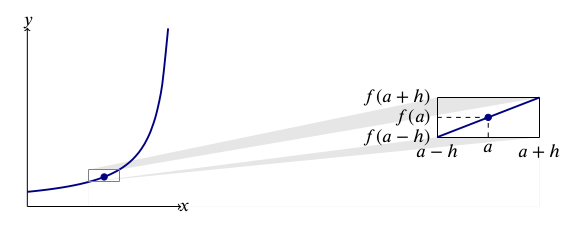
\includegraphics{backupGraph.png}
%% \end{image}


\begin{problem}
  Which of the following approximate the slope of the ``zoomed line''?
  \begin{selectAll}
    \choice{$\frac{(f(a)+h) - f(a)}{(a+h)-a}$}
    \choice[correct]{$\frac{f(a+h) - f(a)}{(a+h)-a}$}
    \choice{$\frac{(f(a)-h) - f(a)}{(a-h)-a}$}
    \choice[correct]{$\frac{f(a-h) - f(a)}{(a-h)-a}$}
    \choice{$\frac{f(a) - (f(a)+h)}{a-(a+h)}$}
    \choice[correct]{$\frac{f(a) - f(a+h)}{a-(a+h)}$}
    \choice{$\frac{f(a) - (f(a)-h)}{a-(a-h)}$}
    \choice[correct]{$\frac{f(a) - f(a-h)}{a-(a-h)}$}
  \end{selectAll}
\end{problem}

\begin{problem}
   Let $f(x) = 3x-1$.  Zoom in on the curve around $a = -2$ so that $h
   = 0.1$.  Use one of the formulations in the problem above to
   approximate the slope of the curve.  The slope of the curve at $a =
   -2$ is approximately\dots \begin{prompt}$\answer{3}$\end{prompt}
\end{problem}

\begin{problem}
   Repeat the previous problem for $f(x) = x^2 - 1$, $a = 0$, and $h =
   0.2$.  Choose a formulation that will give you a positive answer
   for the slope.  The (positive) slope of the curve at $a = 0$ is
   approximately\dots\begin{prompt} $\answer{0.2}$\end{prompt}
\end{problem}


\begin{problem}
   Zoom in on the curve $f(x) = x^2 - 1$ near $x=0$ again.  By looking
   at the graph, what is your best guess for the actual slope of the
   curve at zero?
   \begin{multipleChoice}
     \choice{impossible to say}
     \choice[correct]{zero}
     \choice{one}
     \choice{infinity}
   \end{multipleChoice}
\end{problem}

\begin{xarmaBoost}
  Write down at least \textbf{five} questions for this lecture. After
  you have your questions, label them as ``Level 1,'' ``Level 2,'' or
  ``Level 3'' where:
\begin{description}
\item[Level 1] Means you know the answer, or know exactly how to do
  this problem.
\item[Level 2] Means you think you know how to do the problem.
\item[Level 3] Means you have no idea how to do the problem.
\end{description}
\begin{freeResponse}
\end{freeResponse}
\end{xarmaBoost}



\end{document}
